\documentclass[handout,10pt]{beamer}
%\documentclass[10pt]{beamer}
%\documentclass[draft, 10pt]{beamer}

%\mode<handout>{\beamertemplatesolidbackgroundcolor{black!5}}

 % \textheight 7cm
 %\doublespace
 %\oddsidemargin -1.5cm
 % \evensidemargin +1.5cm
 % \textwidth 12cm
 % \topmargin 0cm

%%%%%\usepackage{times}

%================================================================
\usepackage{ifthen}
\usepackage{color,amsmath,amsfonts,amssymb,epsfig,hyperref,graphicx}
\usepackage{dsfont}
\usepackage[latin1]{inputenc}
\usepackage[T1]{fontenc}
\usepackage[english]{babel}
\usepackage{fancyhdr}
%\usepackage{media9}
\usepackage{tikz}
%\usepackage{pgfplots}

%\usepackage{animate}
%\usepackage{multimedia}
\usepackage{everypage}
\usepackage[absolute,overlay]{textpos}
\usepackage{tikz}

\definecolor{enstrouge}{RGB}{212,65,84}
\definecolor{liteorange}{RGB}{235,226,52}
\definecolor{greenNoise}{RGB}{243,42,255}
\definecolor{LightRed}{rgb}{0.75,0.0325,0}
\definecolor{LightGrey}{rgb}{0.95,0.95,0.95}
\definecolor{Peach}{rgb}{0.98,0.49,0.25}
\definecolor{BurntOrange}{rgb}{0.79,0.37,0}
\definecolor{LightYellow}{rgb}{1,1,0.92}

\definecolor{litegreen}{RGB}{200,255,200}
\definecolor{enstorange}{RGB}{255,214,10}
\definecolor{enstrouge}{RGB}{212,65,84}
\definecolor{grey}{RGB}{204,204,204}
\definecolor{blue}{RGB}{0,0,255}
\definecolor{almostblack}{RGB}{100,100,100}
\definecolor{violet}{rgb}{0.4,0,0.4}
\definecolor{BurntOrange}{rgb}{0.79,0.37,0}
\definecolor{cyan}{RGB}{0,255,255}
\definecolor{magenta}{RGB}{243,42,255}


%================================================================
\mode<presentation> {
  %== theme
% Antibes, Berlin, Bergen, Berkeley,
% Boadilla, boxes, Copenhagen, Darmstadt, Dresden
% Frankfurt, Goettingen, Hannover, Ilmenau, JuanLesPins
% Luebeck, Madrid, Malmoe, Marburg, Montpellier, PaloAlto
% Pittsburgh, Rochester, Singapore, Szeged, Warsaw
  \usetheme{Copenhagen}%[width=0.18\linewidth,]
%%== colortheme
%%albatross, beetle, crane, dolphin, ove, fly, lily
%% orchid, rose, seagull, seahorse, sidebartab, whale
  \usecolortheme{rose}
  % \useoutertheme contient la pose du logo
  %\useoutertheme{default}
  \setbeamercovered{transparent}
}
\setbeamercolor{sidebar}{bg= enstrouge}
\setbeamercolor{structure}{fg= orange}
\setbeamercolor{alerted text}{fg=blue}

\usefonttheme[onlymath]{serif}
%=======================================
\setbeamerfont{page number in head/foot}{size=\large}
 \setbeamercolor{background canvas}{bg=LightYellow} 
 \setbeamertemplate{footline}[frame number]
 
%\pagestyle{fancy}
% \lhead[]{}
% \chead[]{}
% \rhead[]{}
% \lfoot[]{\includegraphics[scale=0.05]{\DIRLOGO/telecomparis}}
% \cfoot[]{\insertframenumber/\inserttotalframenumber}
% \rfoot[]{}

%======================================================================
%=============== NEW COMMANDS =========================================

\newcommand{\figsstit}[2]{
\begin{figure}[hbtp]
\centerline{
    \hbox{ \epsfig{figure={#1}, scale=#2} }
}
\end{figure}}
%===========================
\newcommand{\figscale}[4]{
\begin{figure}[hbtp]
\centerline{
    \hbox{ \epsfig{figure={#1}, scale=#4} }
}
\begin{center}
\parbox{11 cm}
{
    \caption{\protect\small\it  {#2}}
    \label {#3}
}
\end{center}
\end{figure}}
%===========================
\newcommand{\figdims}[5]{
\begin{figure}[hbtp]
\centerline{
    \hbox{ \epsfig{figure={#1}, height=#4cm, width=#5cm} }
}
\begin{center}
\parbox{10cm}
{
    \caption{\protect\small\it  {#2}}
    \label {#3}
}
\end{center}
\end{figure}}
%======================== \def =================
\def\with{\quad \text{with}\quad}
\def\where{\quad \text{where}\quad}
\def\and{\quad \text{and}\quad}
\def\gandl{\renewcommand\arraystretch{0.5}\begin{array}{c}H_{1}\\>\\<\\H_{0}\end{array}}
\def\GLRT{\ensuremath{\text{GLRT}}}
\def\GLRTdet{\ensuremath{\text{GLRT-det}}}
\def\GLRTstoEG{\ensuremath{\text{GLRT-sto-EG}}}
\def\GLRTstoVG{\ensuremath{\text{GLRT-sto-VG}}}
\def\m2{m$^2$}
\def\Fstat{{F\text{-stat}}}

\def\MSC{\text{MSC}}
\def\hMSC{\widehat{\text{MSC}}}

\def\simas{\stackrel{\mathrm{asympt.}}{\sim}}
\def\simiid{\stackrel{\mathrm{i.i.d.}}{\sim}}

% \def\linetext{\noindent
%       \makebox[\textwidth]{\color{orange}
%       {\rule{\textwidth}{1pt}}}}

 \def\linetext{\noindent{\color{orange}\rule{\textwidth}{1pt}
       \\[\dimexpr-\baselineskip+1mm+0pt]
                \rule{\textwidth}{0.5pt}}}

\def\linepaper{\noindent{\color{orange}\rule{\paperwidth}{1pt}
       \\[\dimexpr-\baselineskip+1mm+0pt]
                \rule{\paperwidth}{0.5pt}}}


%==================================================
\newcommand\algo[1]%
{
    \begin{center} %
    \begin{tabular} {||p{10 cm}l ||}%
    \hline
               #1 &  \\
    \hline
    \end{tabular}
    \vspace{12pt}
    \end{center}
}
\def\uB{\underline B}
\def\uD{\underline D}
\def\ur{\underline r}
\def\ux{\underline x}
\def\uX{\underline X}
\def\ug{\underline g}
\def\uw{\underline w}

\def\utheta{\underline \theta}
\def\uzeta{\underline \zeta}


\def\dx{\dot x}
\def\hx{\hat x}
\def\hy{\hat y}
\def\hX{\hat X}
\def\hY{\hat Y}
\def\tx{{\tilde x}}
\def\tX{{\tilde X}}
\def\cX{{\cal X}}


\def\soi{s_{\mathrm{soi}}}
\def\ns{s_{\mathrm{son}}}

\def\ssoi{\utheta_{\mathrm{soi}}}
\def\sns{\utheta_{\mathrm{son}}}
\def\degree{^{\circ}}

\def\cbullet{{\color{orange}\bullet}}

 \newcommand{\prob}[1]{\mathds{P}\left( #1 \right)}
 \newcommand{\esp}[1]{\mathds{E}\left[ #1 \right]}
 \newcommand{\espunder}[2]{\mathds{E}_{#1}\left[ #2 \right]}
 \newcommand{\var}[1]{\mathrm{var}\left( #1 \right)}
 \newcommand{\cov}[1]{\mathrm{Cov}\left( #1 \right)}
 \newcommand{\card}[1]{\left| #1 \right|}
 \newcommand\trace[1]{{\mathrm{Tr}} \left [ #1 \right] }
 \newcommand\diag[1]{{\mathrm{diag}} \left [ #1 \right] }
 \newcommand{\SNR}{\text{SNR}}
 \newcommand{\CRB}{\text{CRB}}
 \newcommand{\MLE}{\text{MLE}}
 \newcommand{\FIM}{\text{FIM}}
 \newcommand{\auc}{\text{AUC}}

\newenvironment{TAB}{\begin{table}[[hbt] \center \leavevmode}{\end{table}}
\newtheorem{propriete}{Propri\'{e}t\'{e} - \thepropriete}
\newtheorem{theoreme}{Th\'{e}or\`{e}me - \thetheoreme}
\newtheorem{definision}{D\'{e}finition - \thedefinision}
\newtheorem{exemple}{Exemple - \theexemple}
\newtheorem{lemme}{Lemme - \thelemme}


\newif\ifBIS \BISfalse 


%=========== LOGO par SLIDE =====================================
\pgfdeclareimage[height=0.6cm]{logoCTBTO}{logoctbto}

%%============================================================================
%\def\thesection{\arabic{section}}
%\def\thefigure{\arabic{figure}}
%\def\theequation{\arabic{equation}}
%\def\theexercice{\arabic{exercice}}
%\def\theequation{\arabic{exercice}.\arabic{equation}}
%%============================================================================
%\newcounter{auxiliaire}
%%%%%%%% comment
%\setcounter{auxiliaire}{\theenumi}
%\end{enumerate}
% TEXTE
%\begin{enumerate}
%\setcounter{enumi}{\theauxiliaire}
%%============================================================================
%\renewcommand\arraystretch{1.6}
%%============================================================================
%\begin{center}
%\renewcommand\arraystretch{1.8}
%\begin{tabular}{|l|l|p{6cm}|}
%\hline
%fonction &  expression & application
%\\
%\hline\hline
%\end{tabular}
%\end{center}
%%============================================================================
%============================================================================
%============= mise en page =================================================
% dans le bandeau inf\'{e}rieur

% Delete this, if you do not want the table of contents to pop up at
% the beginning of each subsection:
%\AtBeginSubsection[]
%{
%  \begin{frame}<beamer>
%    \frametitle{Outline}
%    \tableofcontents[currentsection,currentsubsection]
%  \end{frame}\pageblanche
%}

\setcounter{tocdepth}{1}

\graphicspath{{figures/}}


%%=======================================================
%================= TITRE ===============================
%============================================
\title{Evaluation of the calibration method on a large campaign of measurement}
\author{
 Charbit M.$^{1}$, 
 Doury B.$^{2}$
 Marty J.$^{3}$,
%\\ \vspace{12pt}
%\parbox{20cm}{ 
%{\tiny  (1) maurice.charbit@CTBT.ORG, CTBTO},\\
%{\tiny (2) benoit.doury@CTBT.ORG, CTBTO}\\,
%{\tiny (3) julien.marty@CTBT.ORG, CTBTO} }\vspace{-24pt}
}

%================== debut ==============================
%=======================================================

% \logo{
% \colorbox{litegreen}{\makebox(352,18){\textcolor{black}
% {\normalsize Infrasound Technology Workshop 2015\hspace{10pt}\vspace{10pt}
%  { \hspace{+0.4cm}  \pgfuseimage{logoCTBTO}}}}}}
 \logo{\colorbox{litegreen}
 {\hspace{12pt}\normalsize\color{black}Infrasound Technology Workshop 2015
 \hspace{20pt}\pgfuseimage{logoCTBTO}}\vspace{-0.68cm}\hspace{-0.0cm}}


 \bibliographystyle{plain} 

\begin{document}
 \sloppy
%=======================================================
%=======================================================
%\begin{frame}
%\frametitle{Short outline}
% \tableofcontents
%\end{frame}

%=======================================================
%=======================================================
\begin{frame}
\maketitle
\end{frame}


 \section{Introduction}
%=======================================================
%=======================================================
\begin{frame}
 \frametitle{IMS study}
 In the framework of the calibration project, a study has been conducted by the 
 IMS that provides some theoretical and practical results:
 \begin{itemize}
 \item
 determining closed form expression for the asymptotic distributions of the estimators,
 \item
sizing a statistic for testing  the magnitude square coherence (MSC) level,
 \item
 introducing a weighted estimator of the sensor under test (SUT) response based on the estimated value of the MSC estimator variance,
 \item
 proposal of a filter bank analysis for the SUT estimation,
 \item
 providing a simple wind coherence model which explains an observed artefact of the noise reduction system (NRS),
 \item
{\color{red} Evaluation on a very large campaign of measurement on IS26}
 \end{itemize}
 
  \bigskip
  
This presentation mainly focuses on the last item
 
\end{frame}
%=======================================================
%=======================================================
%=======================================================
\begin{frame}
\frametitle{Typical condition of measurement}

\figsstit{fulltestbedIS26-eps-converted-to.pdf}{0.5}

\vspace{-24pt}
$$\widehat{SUT}\approx \dfrac{\widehat{SUU}}{\widehat{SUR}}\times SREF$$



\begin{itemize}
\item
objective: calibrate the system under test (SUT), i.e. NRS+sensor.
\item
two kinds of signals: acoustic meaning about 300 m/s, and non acoustic, typically wind, meaning about 3 m/s,
\item
non spatially coherent signals are said "noise''.
\item
acoustic signals  is  spatially coherent regarding the size of the SUT. 
\end{itemize}


\end{frame}
%=======================================================
%=======================================================
%%=======================================================
%\begin{frame}
%\frametitle{Main schema - II}
%
%\figsstit{schema-of-observation-eps-converted-to.pdf}{0.55}
%
%\vspace{-12pt}
%
%A few remarks:
%\begin{itemize}
%\item
%two kinds of signals: acoustic meaning about 300 m/s, and non acoustic meaning about 5 m/s,
%\item
%$s(t)$ is said \emph{common or coherent} because this signal is assumed to be spatially coherent w.r.t. the size of the SUT,
%\end{itemize}
%
%\end{frame}
%=======================================================
%=======================================================
%=======================================================
\begin{frame}
\frametitle{NRS effect}

The ratio $\dfrac{v_{\mathrm{wind}}}{f}$ can be interpreted as a wavelength. Therefore

 
\bigskip

\begin{tabular}{cl}
\hspace{-1cm}
\begin{minipage}{6cm}
\begin{itemize}
\item
{\color{red}at very low frequency}, 
{\tiny the wind appears as spatially coherent for all SUT inlets and SREF inlet. Therefore everything occurs as there is NO noise, and the MSC is almost 1},
\item
{\color{red}at high frequency},  
{\tiny the wind appears as spatially NON coherent. Therefore the NRS plays its role to reduce the noise},
\item
{\color{red}at the mid frequency range}, 
{\tiny a small part of the wind appears as  spatially coherent for near inlets. Therefore a dip artefact is observed}.
\end{itemize}
\end{minipage}
&
\begin{minipage}{7.5cm}
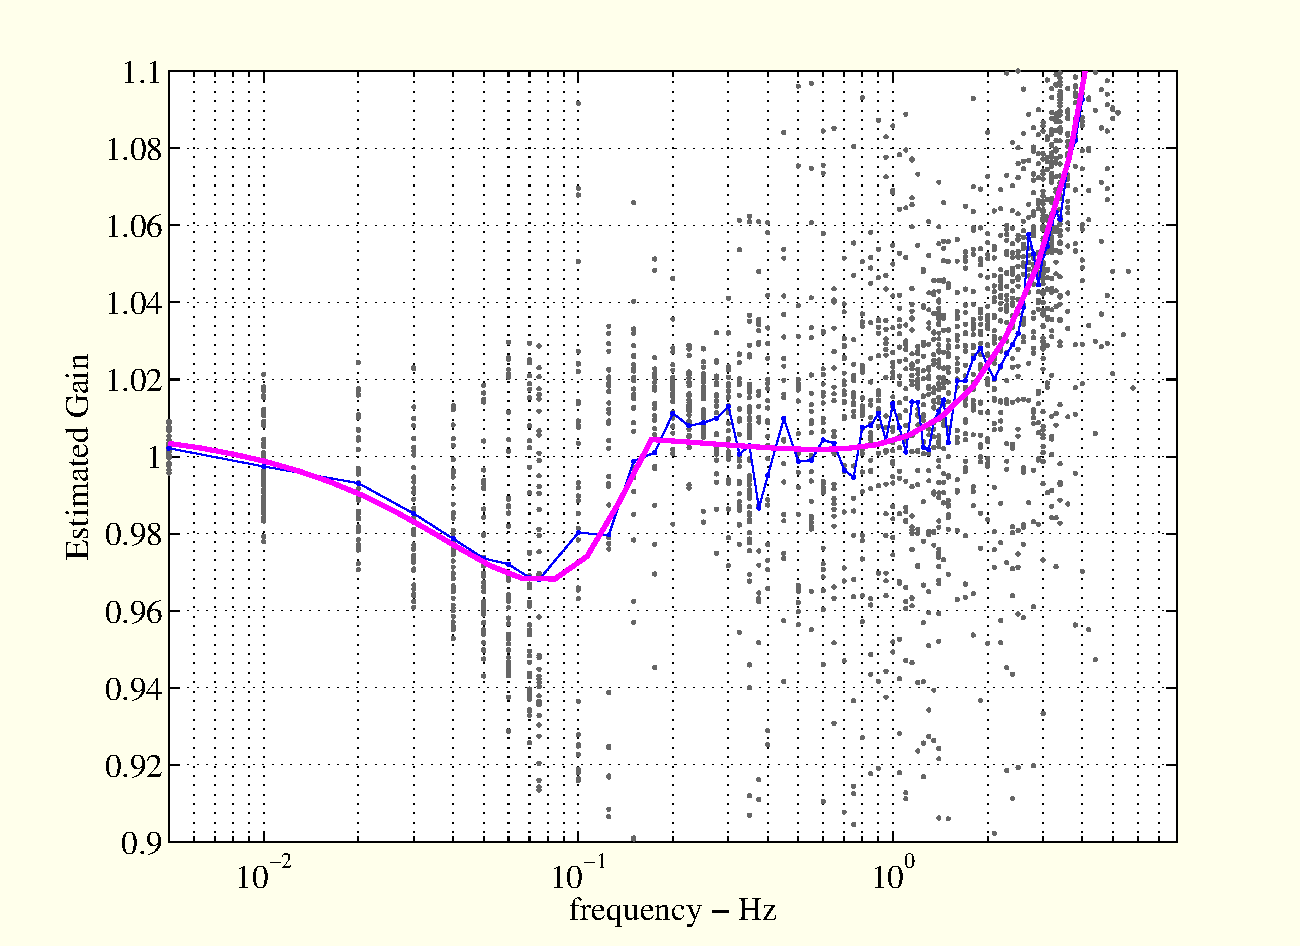
\includegraphics[scale=0.28]{3zones3.pdf}
\end{minipage}
\end{tabular}


\end{frame}
%=======================================================
%=======================================================
%=======================================================
\begin{frame}
\frametitle{Manage the stationarity}

Spectrum analysis requires stationarity. In high frequencies the duration where we can expect stationarity can be considered smaller. Hence the use of a filter bank. An example is given below.

\figsstit{filterbank-eps-converted-to.pdf}{0.55}


\end{frame}
%=======================================================
\section{Campaign measurement results}
%=======================================================
%=======================================================
\begin{frame}
\frametitle{Results on confidence interval}
\begin{tabular}{cc}
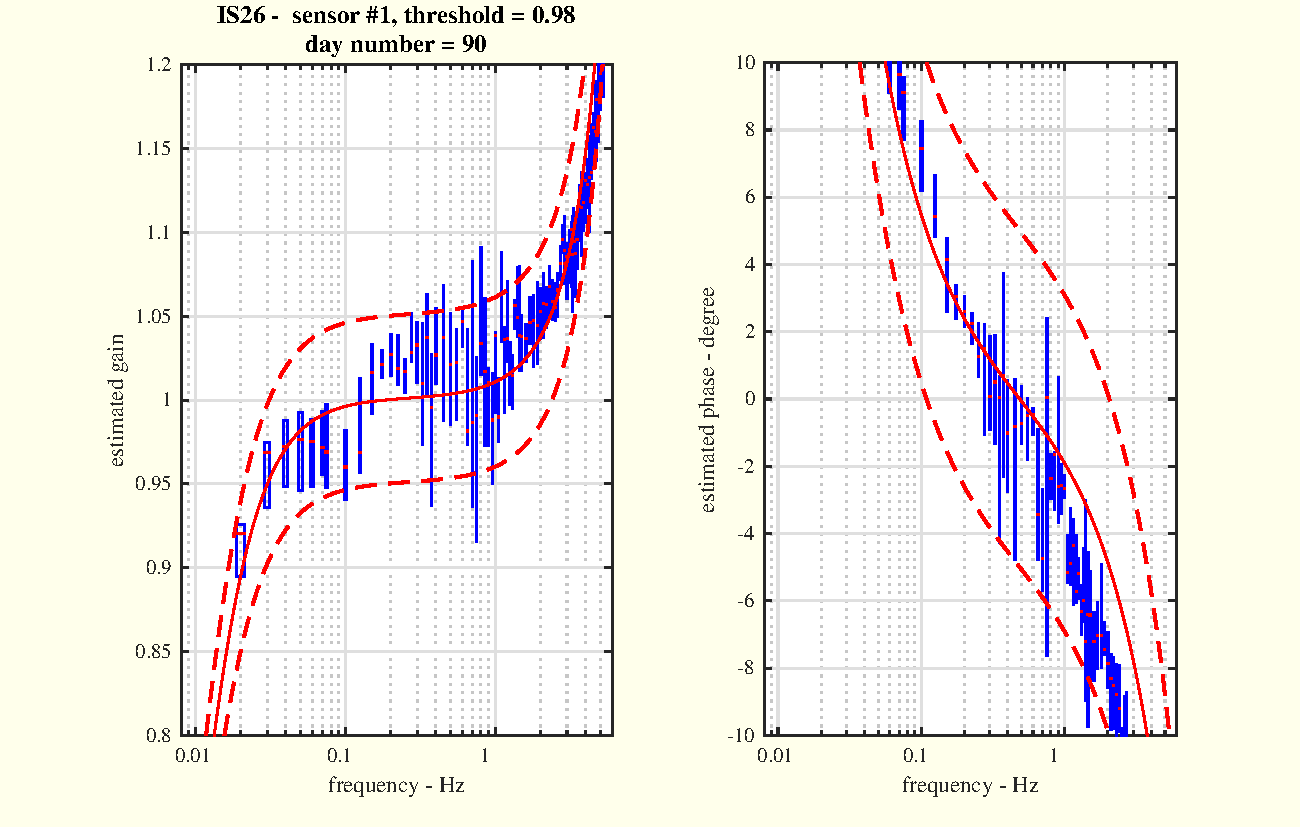
\includegraphics[scale=0.25]{3monthsonIS26SUTboxplot1-eps-converted-to.pdf}
&
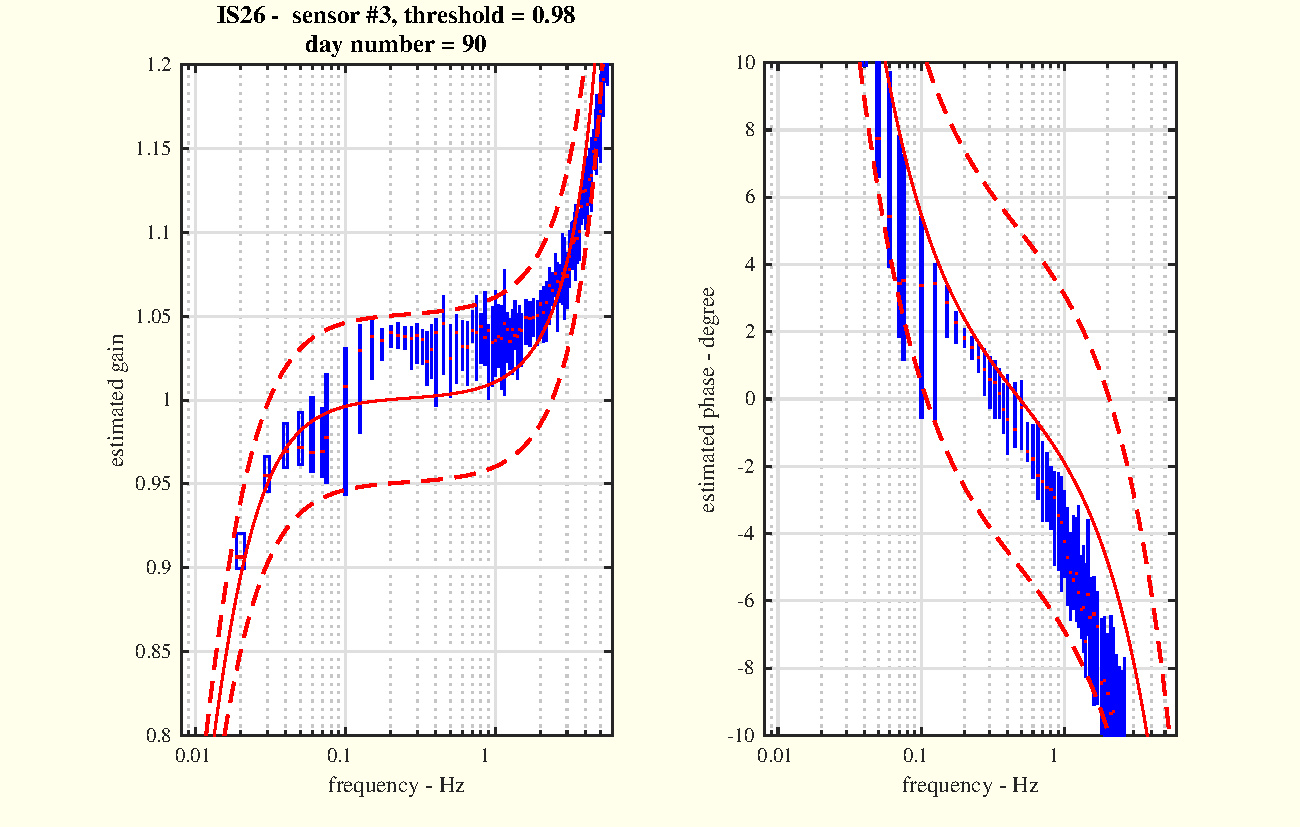
\includegraphics[scale=0.25]{3monthsonIS26SUTboxplot3-eps-converted-to.pdf}
\\
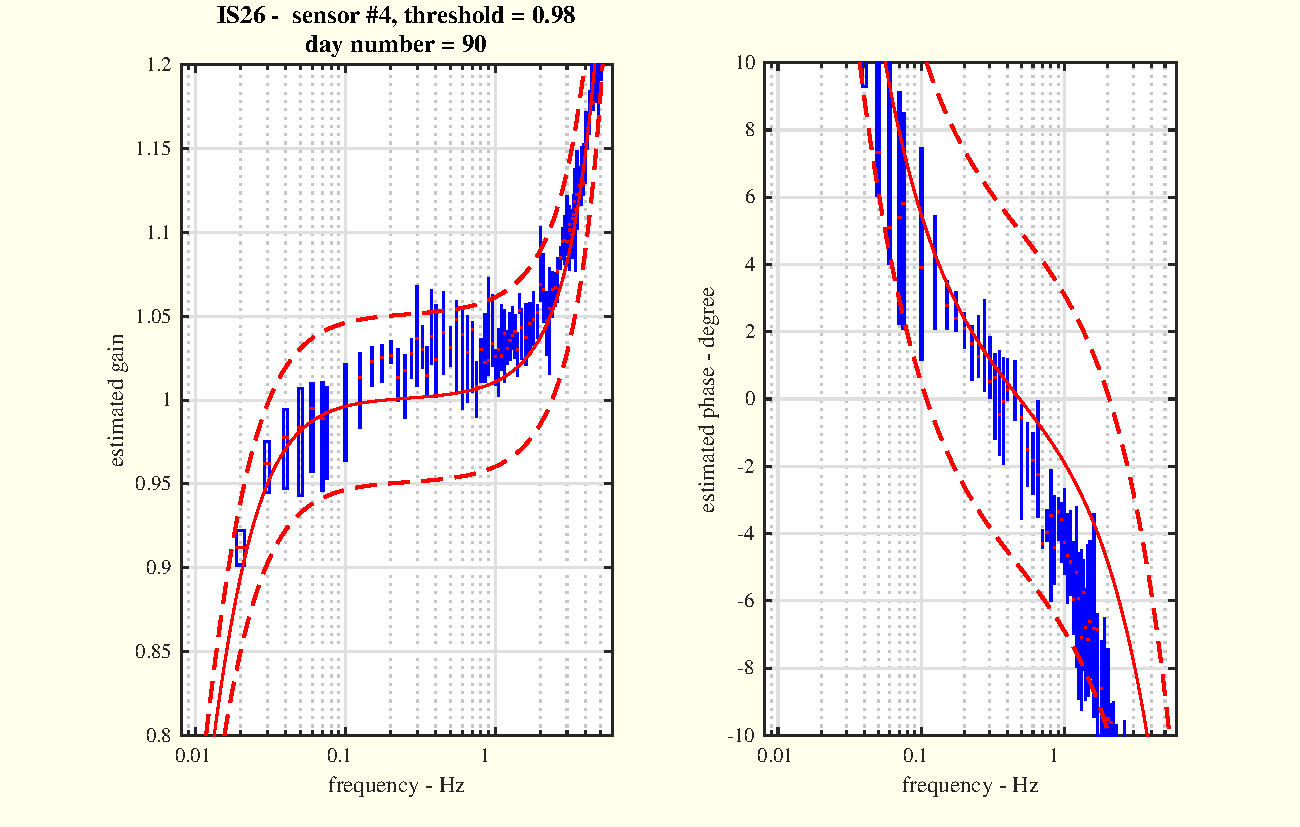
\includegraphics[scale=0.25]{3monthsonIS26SUTboxplot4-eps-converted-to.pdf}
&
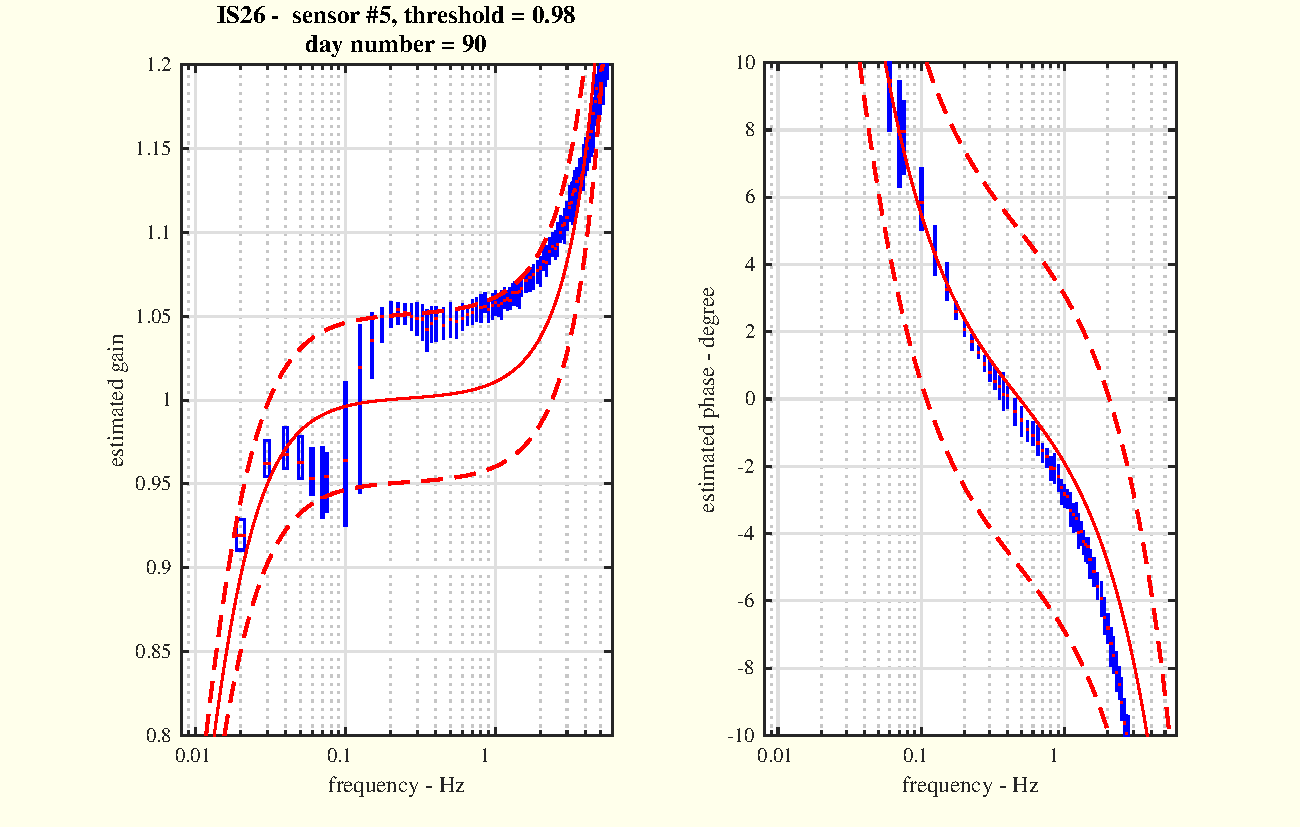
\includegraphics[scale=0.25]{3monthsonIS26SUTboxplot5-eps-converted-to.pdf}
\end{tabular}
\end{frame}
%%=======================================================
%%=======================================================
%\begin{frame}
%\frametitle{Results on confidence interval}
%
%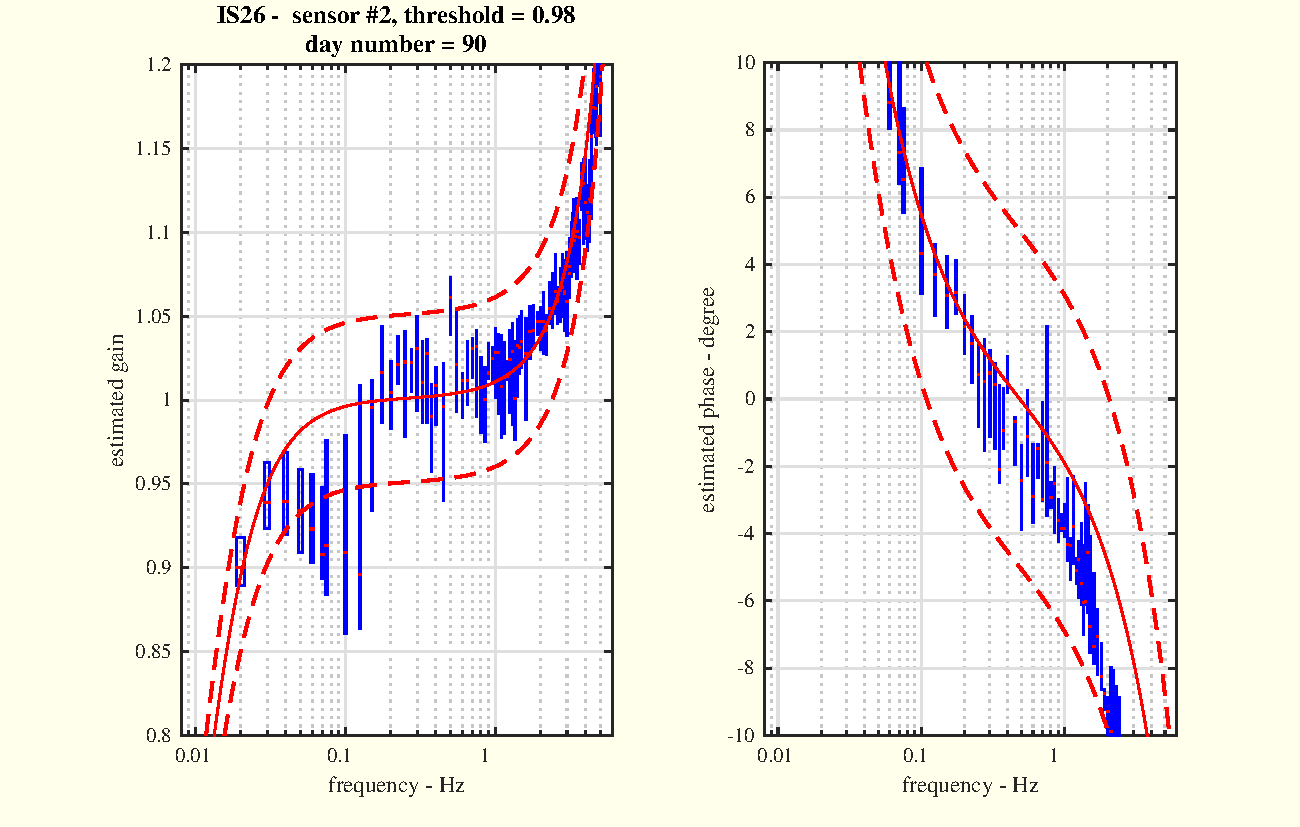
\includegraphics[scale=0.5]{3monthsonIS26SUTboxplot2-eps-converted-to.pdf}
%
%\end{frame}
%%=======================================================
%%=======================================================
%\begin{frame}
%\frametitle{Results on confidence interval}
%
%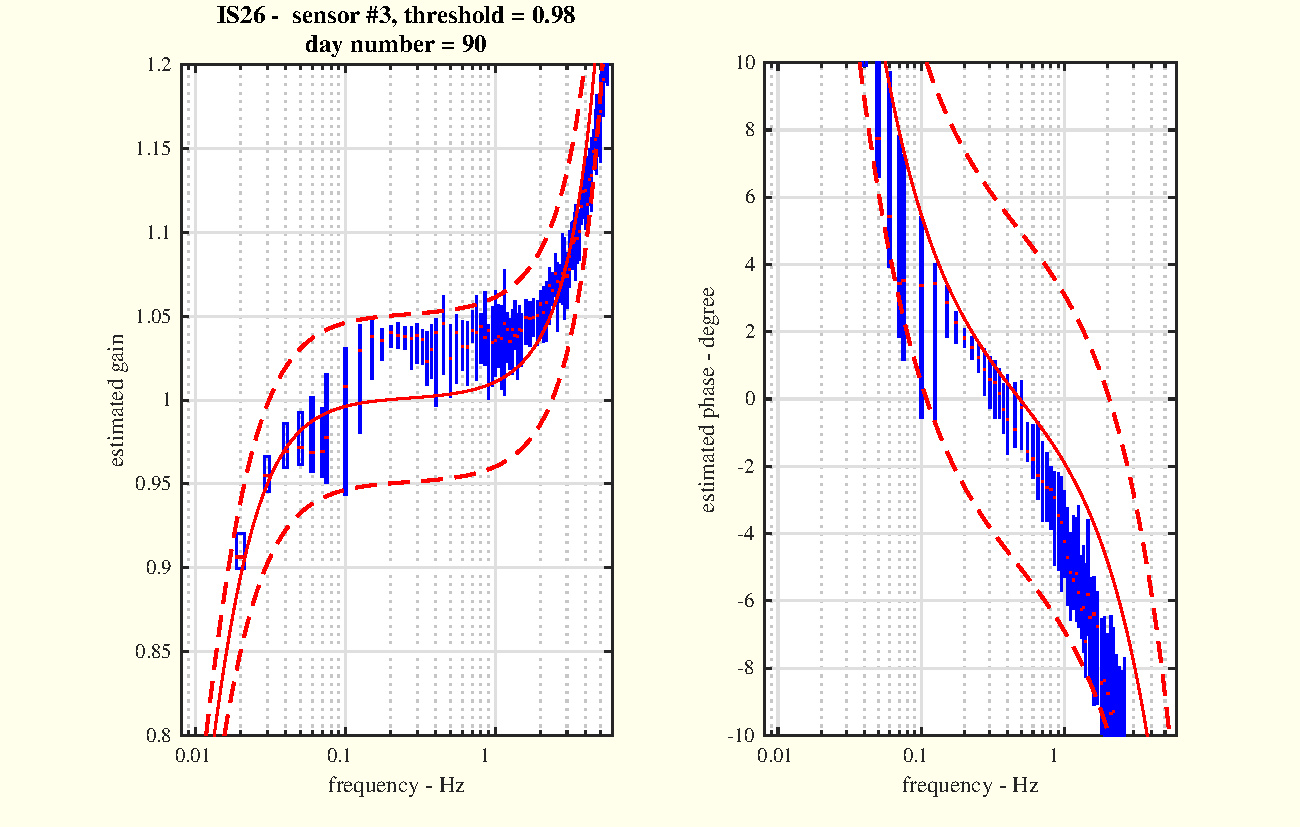
\includegraphics[scale=0.5]{3monthsonIS26SUTboxplot3-eps-converted-to.pdf}
%
%\end{frame}
%%=======================================================
%%=======================================================
%\begin{frame}
%\frametitle{Results on confidence interval}
%
%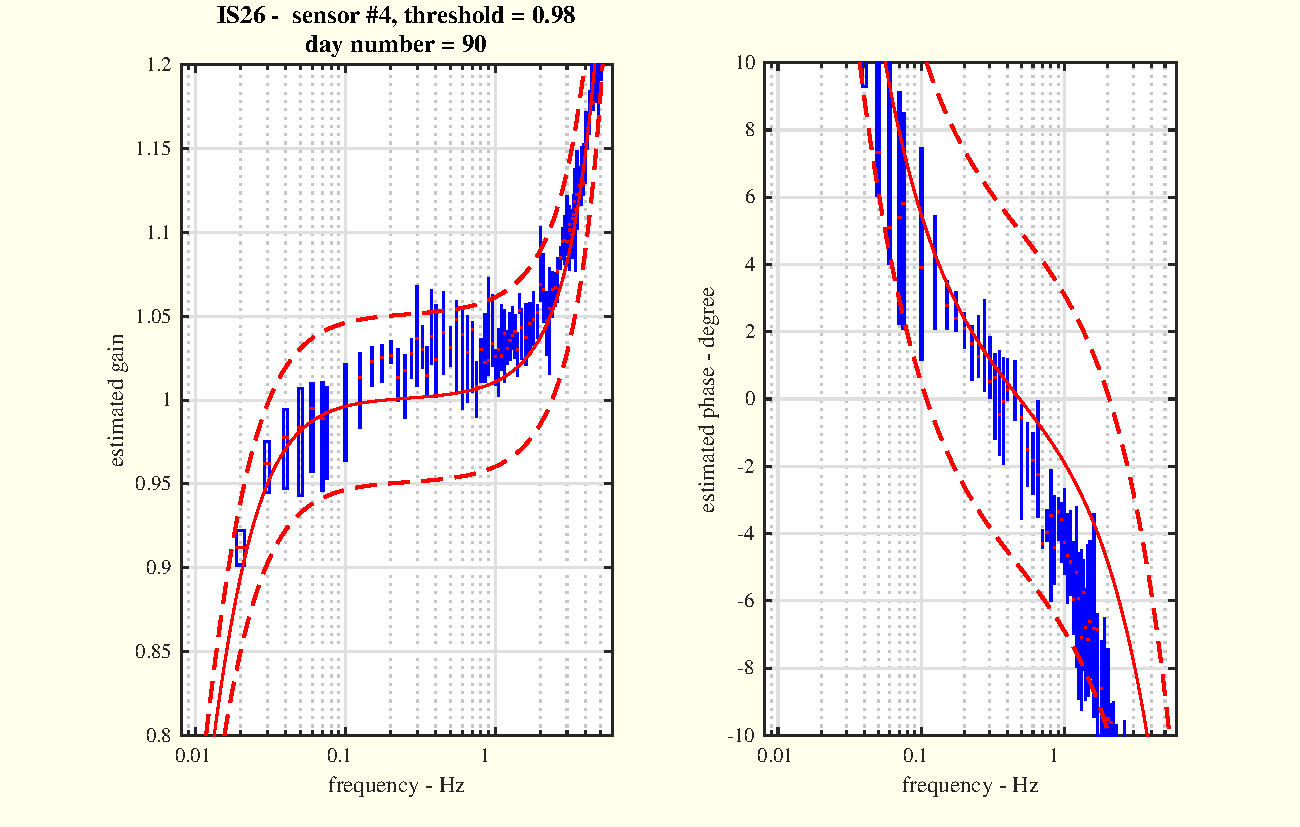
\includegraphics[scale=0.5]{3monthsonIS26SUTboxplot4-eps-converted-to.pdf}
%
%\end{frame}
%%=======================================================
%%=======================================================
%\begin{frame}
%\frametitle{Results on confidence interval}
%
%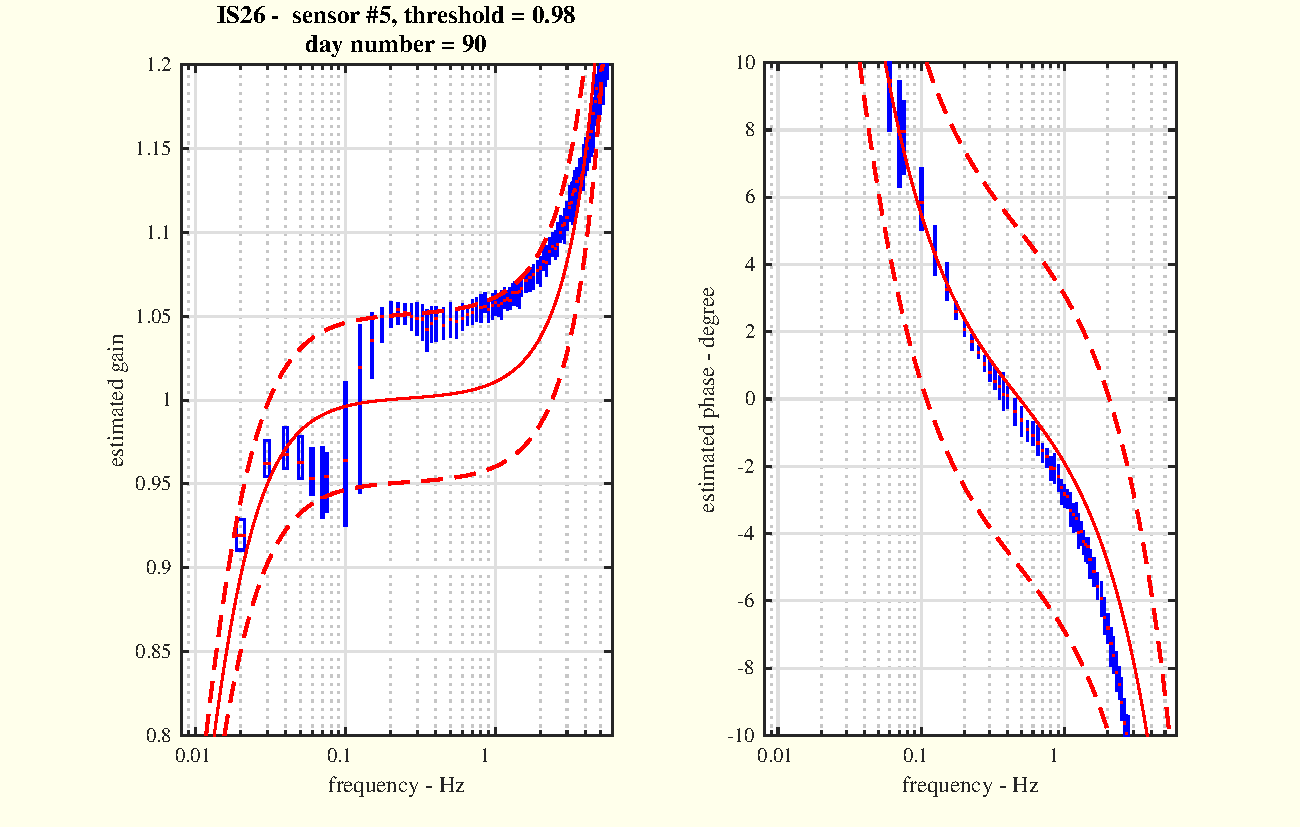
\includegraphics[scale=0.5]{3monthsonIS26SUTboxplot5-eps-converted-to.pdf}
%
%\end{frame}
%%=======================================================
%%=======================================================
%\begin{frame}
%\frametitle{Results on confidence interval}
%
%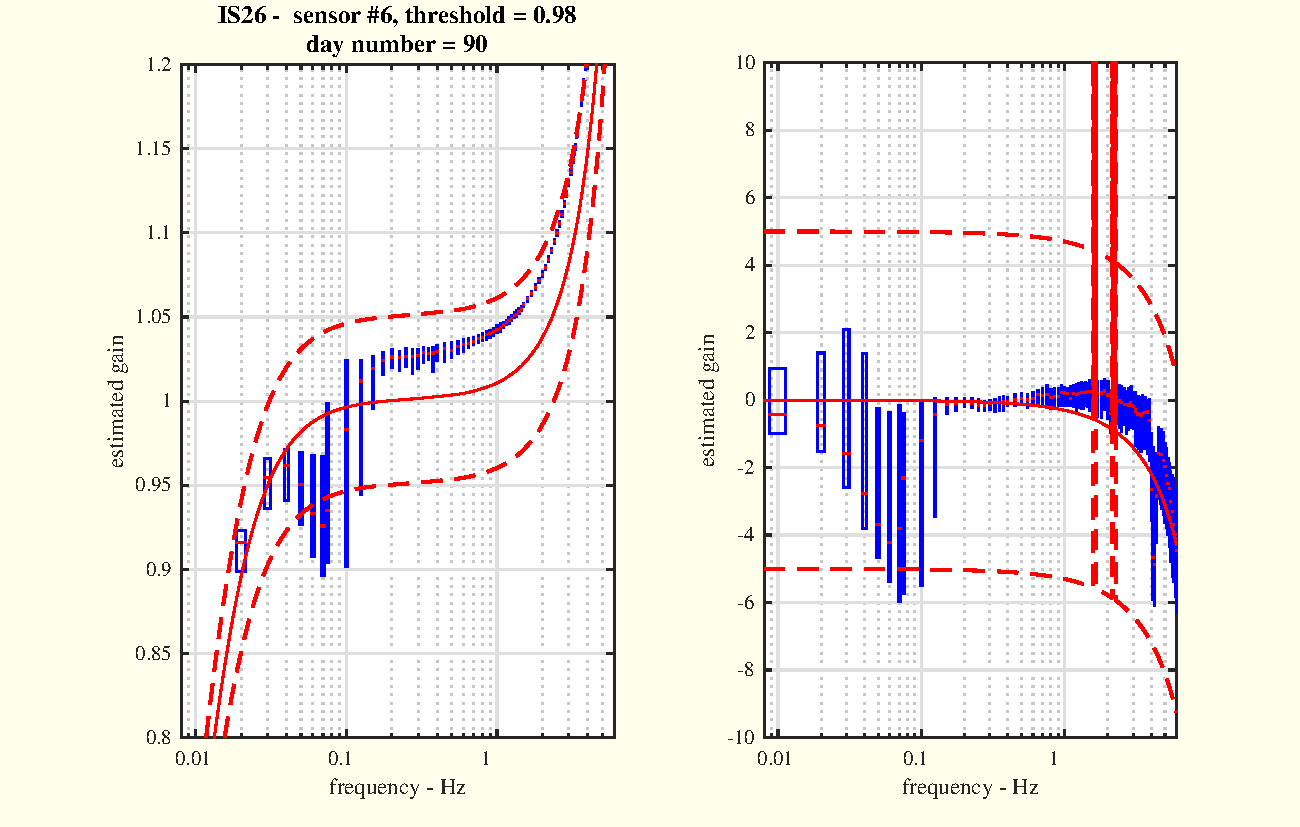
\includegraphics[scale=0.5]{3monthsonIS26SUTboxplot6-eps-converted-to.pdf}
%
%\end{frame}
%%=======================================================
%%=======================================================
%\begin{frame}
%\frametitle{Results on confidence interval}
%
%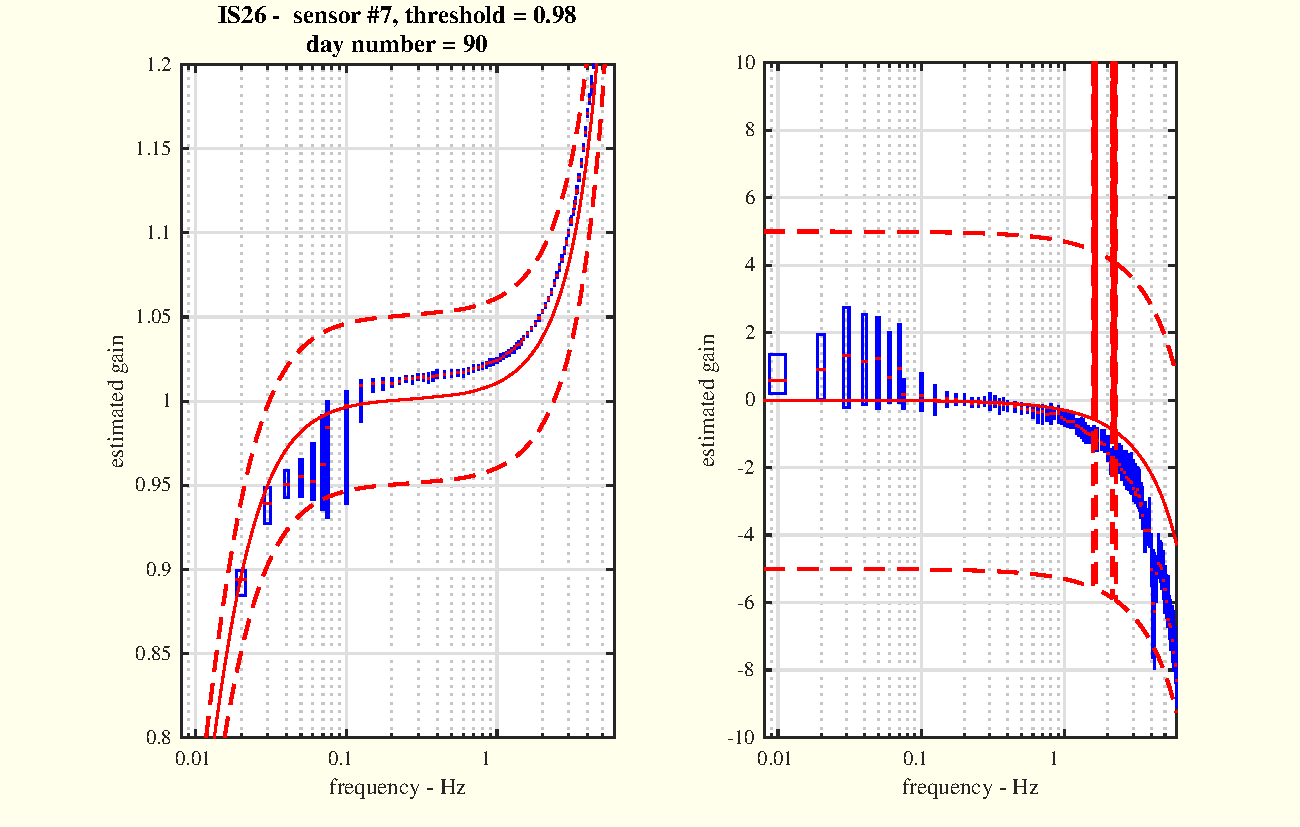
\includegraphics[scale=0.5]{3monthsonIS26SUTboxplot7-eps-converted-to.pdf}
%
%\end{frame}
%%=======================================================
%%=======================================================
%\begin{frame}
%\frametitle{Results on confidence interval}
%
%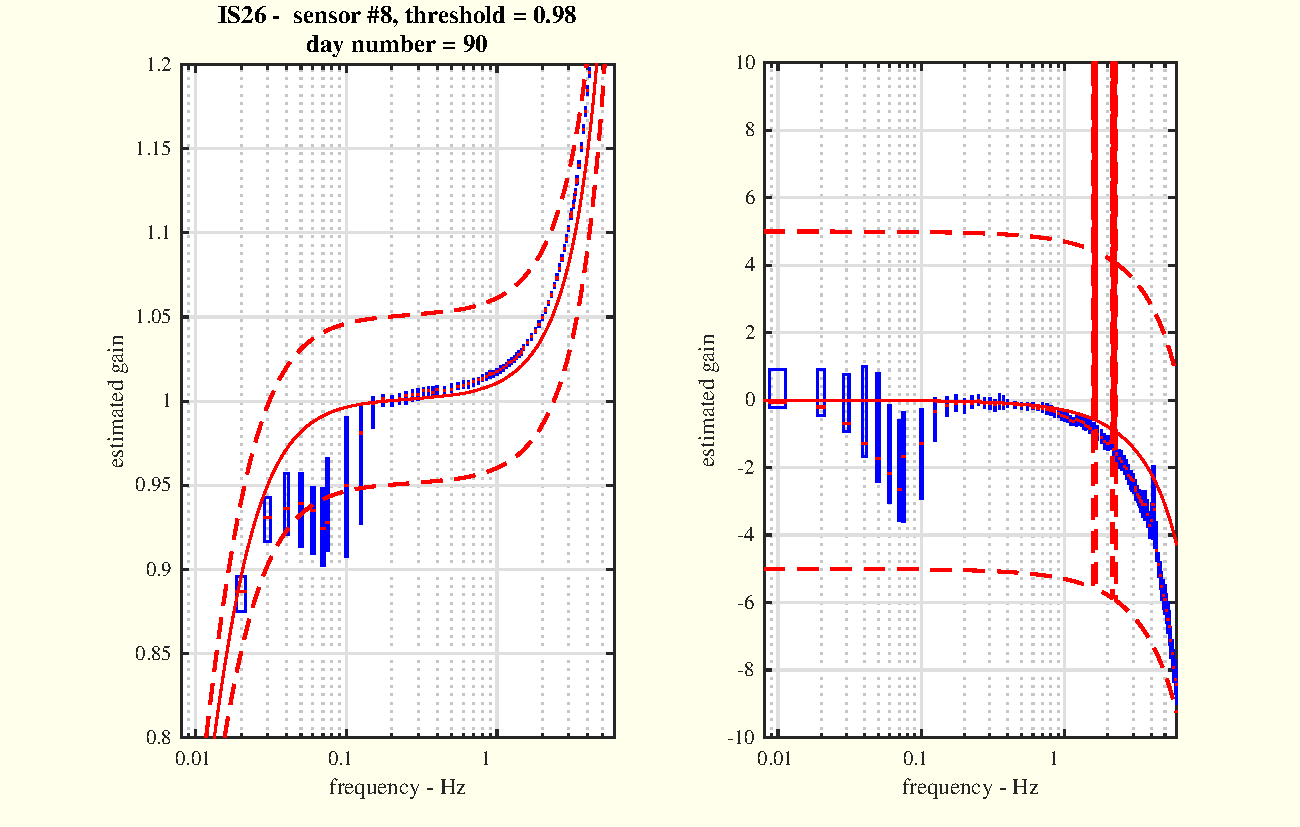
\includegraphics[scale=0.5]{3monthsonIS26SUTboxplot8-eps-converted-to.pdf}
%
%\end{frame}
%=======================================================
%=======================================================
\begin{frame}
\frametitle{Temporal variability at the 1 Hz frequency value}
\begin{tabular}{cc}
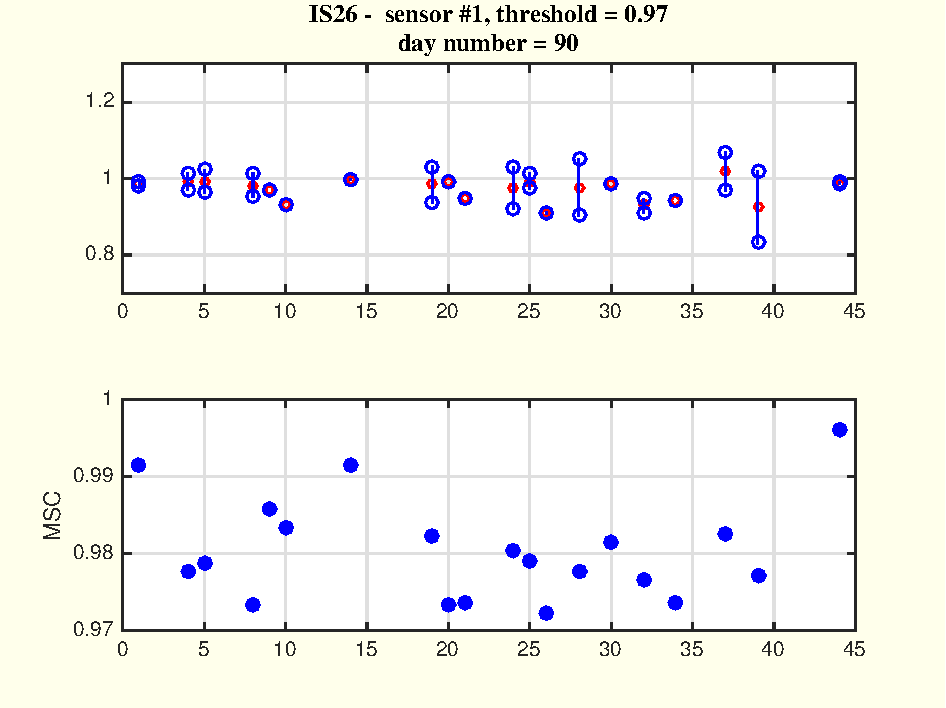
\includegraphics[scale=0.3]{evolutionon1atfreq1-eps-converted-to.pdf}
&
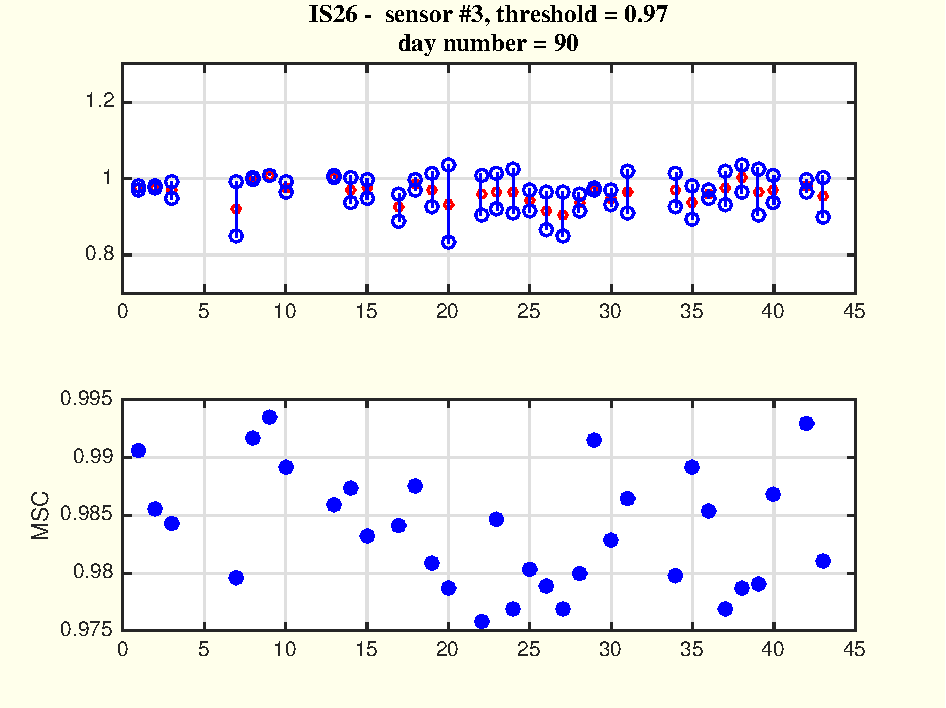
\includegraphics[scale=0.3]{evolutionon3atfreq1-eps-converted-to.pdf}
\\
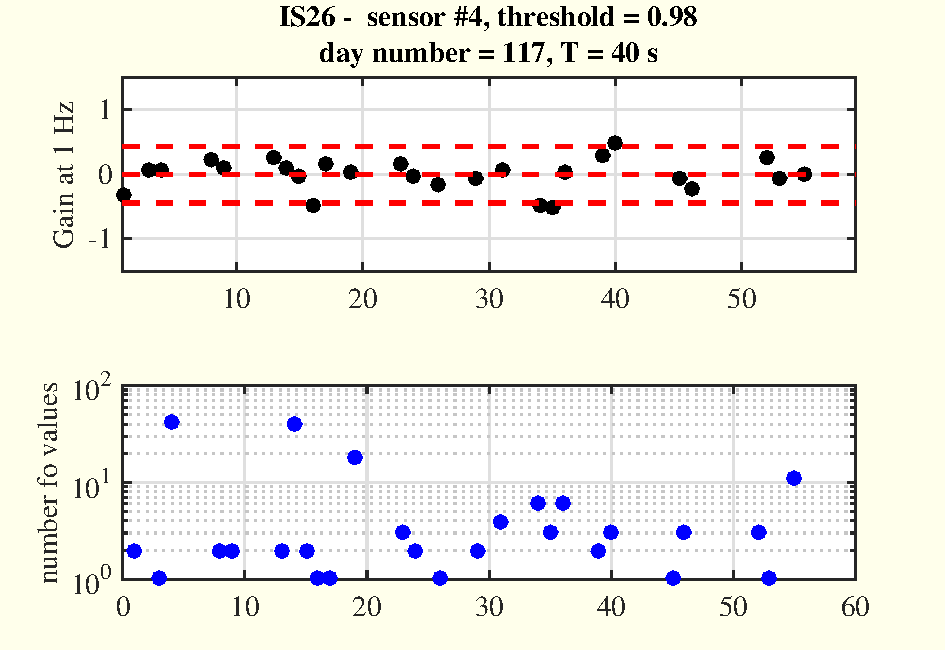
\includegraphics[scale=0.3]{evolutionon4atfreq1-eps-converted-to.pdf}
&
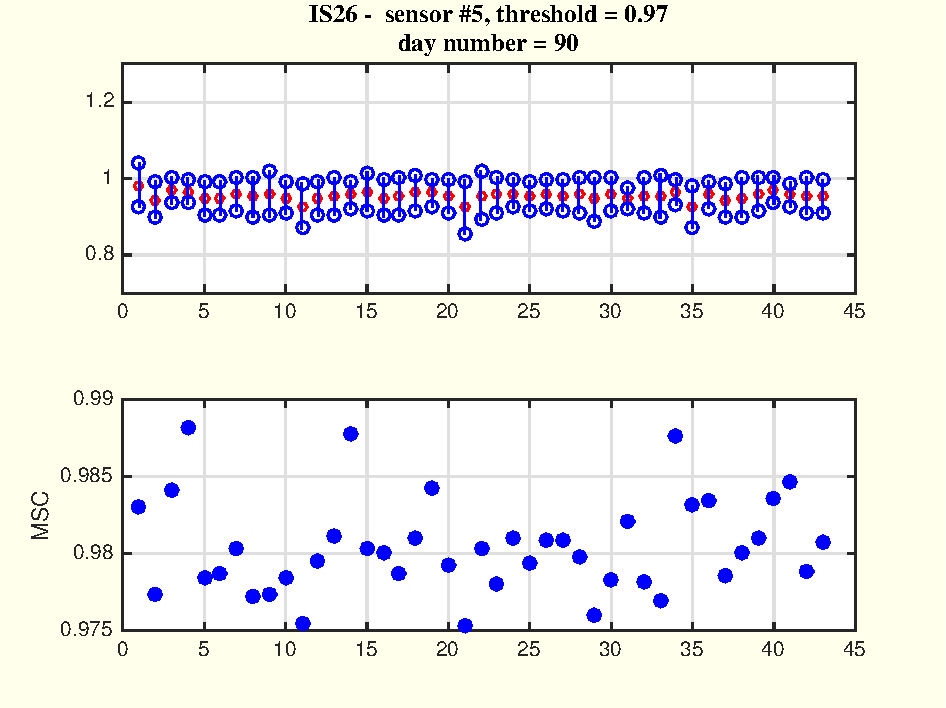
\includegraphics[scale=0.3]{evolutionon5atfreq1-eps-converted-to.pdf}
\end{tabular}
\end{frame}
%%=======================================================
%%=======================================================
%\begin{frame}
%\frametitle{Temporal variability at the 1 Hz frequency value}
%
%\figsstit{evolutionon2atfreq1-eps-converted-to.pdf}{0.55}
%\end{frame}
%%=======================================================
%%=======================================================
%\begin{frame}
%\frametitle{Temporal variability at the 1 Hz frequency value}
%
%\figsstit{evolutionon3atfreq1-eps-converted-to.pdf}{0.55}
%\end{frame}
%%=======================================================
%%=======================================================
%\begin{frame}
%\frametitle{Temporal variability at the 1 Hz frequency value}
%
%\figsstit{evolutionon4atfreq1-eps-converted-to.pdf}{0.55}
%\end{frame}
%=======================================================
%=======================================================
%\begin{frame}
%\frametitle{Temporal variability at the 1 Hz frequency value}
%
%\figsstit{evolutionon5atfreq1-eps-converted-to.pdf}{0.55}
%\end{frame}
%%=======================================================
%%=======================================================
\begin{frame}
\frametitle{Conclusion}

The experimental results obtained during 3 months on IS26 fully validate the calibration method.

\end{frame}
%=======================================================
%=======================================================

\begin{frame}
\begin{center}
{\large THANKS FOR YOUR ATTENTION}
\end{center}
\end{frame}

\end{document}





%=======================================================
%=======================================================
\begin{frame}\frametitle{Rks}
{\tiny
\begin{center}
\hspace{-0.8 cm}
\fbox{$X_1,\cdots,X_{2000}$}\ \fbox{$X_{2001},\cdots,X_{4000}$}\ %
\fbox{$X_{4001},\cdots,X_{6000}$}\ \fbox{$X_{6001},\cdots,X_{8000}$}\
%
\fbox{$X_{8001},\cdots,X_{10000}$} \\
\hspace{-1. cm}
\fbox{$X_{1001},\cdots,X_{3000}$}\ \fbox{$X_{3001},\cdots,X_{5000}$}\
%
\fbox{$X_{5001},\cdots,X_{7000}$}\ \fbox{$X_{7001},\cdots,X_{9000}$}
\end{center}
}
\begin{itemize}
\item
We have $N=2000$ time samples leading to a resolution of $F_s/N=0.01$ Hz. 
Therefore there is a possibility to decimate if the bandwidth is $B<0.01$.
But for sake of simplicity, we keep the common value $F_s$ to all filters of the bank.
\item
For each frequency bin, an averaging is applied on the $L=9$ segments. If a few number of bins is required the fft algorithm is not needed.
\end{itemize}
\end{frame}
